% Options for packages loaded elsewhere
\PassOptionsToPackage{unicode}{hyperref}
\PassOptionsToPackage{hyphens}{url}
%
\documentclass[
]{article}
\usepackage{amsmath,amssymb}
\usepackage{lmodern}
\usepackage{iftex}
\ifPDFTeX
  \usepackage[T1]{fontenc}
  \usepackage[utf8]{inputenc}
  \usepackage{textcomp} % provide euro and other symbols
\else % if luatex or xetex
  \usepackage{unicode-math}
  \defaultfontfeatures{Scale=MatchLowercase}
  \defaultfontfeatures[\rmfamily]{Ligatures=TeX,Scale=1}
\fi
% Use upquote if available, for straight quotes in verbatim environments
\IfFileExists{upquote.sty}{\usepackage{upquote}}{}
\IfFileExists{microtype.sty}{% use microtype if available
  \usepackage[]{microtype}
  \UseMicrotypeSet[protrusion]{basicmath} % disable protrusion for tt fonts
}{}
\makeatletter
\@ifundefined{KOMAClassName}{% if non-KOMA class
  \IfFileExists{parskip.sty}{%
    \usepackage{parskip}
  }{% else
    \setlength{\parindent}{0pt}
    \setlength{\parskip}{6pt plus 2pt minus 1pt}}
}{% if KOMA class
  \KOMAoptions{parskip=half}}
\makeatother
\usepackage{xcolor}
\usepackage[margin=1in]{geometry}
\usepackage{graphicx}
\makeatletter
\def\maxwidth{\ifdim\Gin@nat@width>\linewidth\linewidth\else\Gin@nat@width\fi}
\def\maxheight{\ifdim\Gin@nat@height>\textheight\textheight\else\Gin@nat@height\fi}
\makeatother
% Scale images if necessary, so that they will not overflow the page
% margins by default, and it is still possible to overwrite the defaults
% using explicit options in \includegraphics[width, height, ...]{}
\setkeys{Gin}{width=\maxwidth,height=\maxheight,keepaspectratio}
% Set default figure placement to htbp
\makeatletter
\def\fps@figure{htbp}
\makeatother
\setlength{\emergencystretch}{3em} % prevent overfull lines
\providecommand{\tightlist}{%
  \setlength{\itemsep}{0pt}\setlength{\parskip}{0pt}}
\setcounter{secnumdepth}{5}
\usepackage{booktabs}
\usepackage{longtable}
\usepackage{array}
\usepackage{multirow}
\usepackage{wrapfig}
\usepackage{float}
\usepackage{colortbl}
\usepackage{pdflscape}
\usepackage{tabu}
\usepackage{threeparttable}
\usepackage{threeparttablex}
\usepackage[normalem]{ulem}
\usepackage{makecell}
\usepackage{xcolor}
\ifLuaTeX
  \usepackage{selnolig}  % disable illegal ligatures
\fi
\usepackage[]{natbib}
\bibliographystyle{plainnat}
\IfFileExists{bookmark.sty}{\usepackage{bookmark}}{\usepackage{hyperref}}
\IfFileExists{xurl.sty}{\usepackage{xurl}}{} % add URL line breaks if available
\urlstyle{same} % disable monospaced font for URLs
\hypersetup{
  pdftitle={Social learning by type-token frequency - stimulus preparation},
  pdfkeywords={Keywords},
  hidelinks,
  pdfcreator={LaTeX via pandoc}}

\title{Social learning by type-token frequency - stimulus preparation}
\author{Ansgar D. Endress\\
City, University of London}
\date{}

\begin{document}
\maketitle
\begin{abstract}
Abstract (to be written)
\end{abstract}

\hypertarget{stimulus-selection}{%
\section{Stimulus selection}\label{stimulus-selection}}

\hypertarget{faces}{%
\subsection{Faces}\label{faces}}

We selected the stimuli from the 2,222 annotated face images in
\citep{Bainbridge2013}. For each gender and valency, we need 4 (sets)
\(\times\) 3 (actions per set) \(\times\) 6 (actions) = 120 faces. We
thus need 360 faces per gender.

We selected face photographs for non-famous persons with an image
quality rating of at least 3, an estimated age between 20 and 60, and
memorability (operationalized as \citep{ZhangMueller2005} version of
\(A^\prime\)) between the 25\% and 85\% quantile. This yielded 278 and
380 pictures for females and males, respectively.We then randomly
selected the required number of faces from this initial set. 216 faces
were randomly selected for each gender.

The distribution of various properties of the faces is shown in Figure
\ref{fig:plot-face-attributes-nonfamous}.

\begin{figure}

{\centering 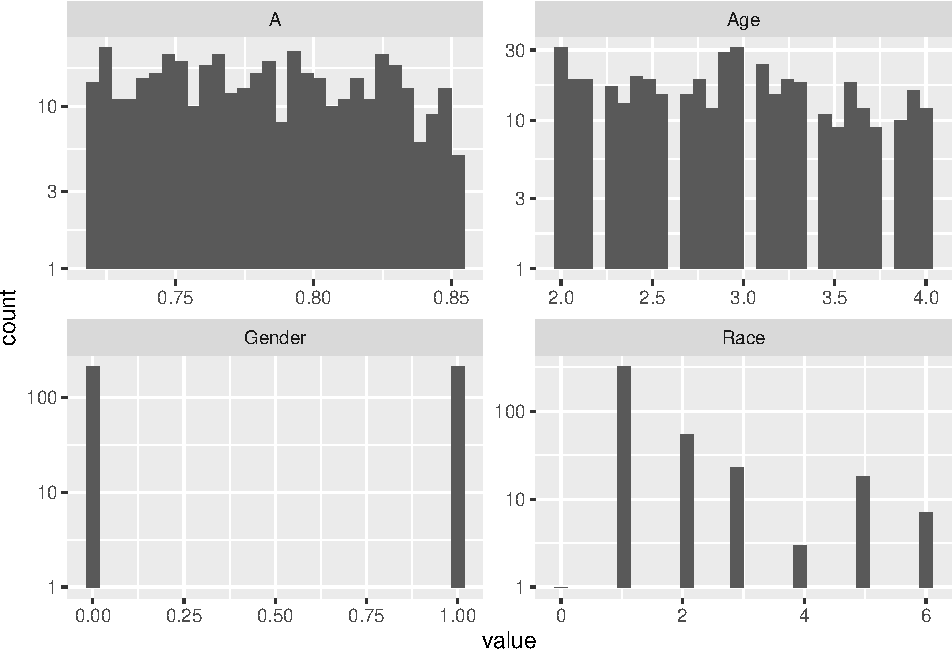
\includegraphics[width=0.8\linewidth]{social_learning_type_token_sequential_files/figure-latex/plot-face-attributes-nonfamous-1} 

}

\caption{Distribution of various properties of the faces in the database after filtering. See main text for the filters.}\label{fig:plot-face-attributes-nonfamous}
\end{figure}

\clearpage

\hypertarget{counterbalancing}{%
\section{Counterbalancing}\label{counterbalancing}}

We will use behaviors performed 6 times by the same individual or once
by 6 different individuals, as well as an action performed once by one
individual. To make sure that responses are not based on prior estimates
of the prevalence of individual actions, the behaviors will be
counterbalanced across participants.

We need 12 actions per valency. If we use 3 actions per trial, this
gives us 4 trials. As shown in Table
\ref{tab:counterbalancing-frequency-conditions-print}, the role of the
actions in the trials will be counterbalanced within participants.
Further, valency will be counterbalanced across participants, with each
participant seenig only one valency.

\begin{table}

\caption{\label{tab:counterbalancing-frequency-conditions-print}Counterbalancing of the roles of actions. Separately for each valency, actions were organized into 4 sets. Across blocks, each action of a set was presented as the high type-frequency, low type-frequency and single occurrence action.}
\centering
\begin{tabular}[t]{lllll}
\toprule
Role & Set 1 & Set 2 & Set 3 & Set 4\\
\midrule
\addlinespace[0.3em]
\multicolumn{5}{l}{\textbf{Condition 1}}\\
\hspace{1em}High Type-Frequency & Action 1 & Action 4 & Action 7 & Action 10\\
\hspace{1em}Low Type-Frequency & Action 2 & Action 5 & Action 8 & Action 11\\
\hspace{1em}Single occurrence & Action 3 & Action 6 & Action 9 & Action 12\\
\addlinespace[0.3em]
\multicolumn{5}{l}{\textbf{Condition 2}}\\
\hspace{1em}High Type-Frequency & Action 2 & Action 5 & Action 8 & Action 11\\
\hspace{1em}Low Type-Frequency & Action 3 & Action 6 & Action 9 & Action 12\\
\hspace{1em}Single occurrence & Action 1 & Action 4 & Action 7 & Action 10\\
\addlinespace[0.3em]
\multicolumn{5}{l}{\textbf{Condition 3}}\\
\hspace{1em}High Type-Frequency & Action 3 & Action 6 & Action 9 & Action 12\\
\hspace{1em}Low Type-Frequency & Action 1 & Action 4 & Action 7 & Action 10\\
\hspace{1em}Single occurrence & Action 2 & Action 5 & Action 8 & Action 11\\
\bottomrule
\end{tabular}
\end{table}

We will administer all three conditions to all participants; all 12
blocks appear in random order. Additionally, for each participant, half
the blocks will use female face, and half male faces. For half of the
participants, Sets 1 and 2 will be presented with male faces and Sets 3
and 4 with female faces. For the remaining participants, this will be
inverted.

\begin{table}

\caption{\label{tab:counterbalancing-gender-define}Counterbalancing. The valency of the action is counter-balanced across participants. Within each valency, the gender of the face the actions are combined to is counterbalanced across participants, giving 3 groups in total.}
\centering
\begin{tabular}[t]{lrrrl}
\toprule
valence & valenceSubjectGroup & genderSubjectGroup & set & faceGender\\
\midrule
\addlinespace[0.3em]
\multicolumn{5}{l}{\textbf{Participant Group 1}}\\
\hspace{1em}bad & 1 & 1 & 1 & male\\
\hspace{1em}bad & 1 & 1 & 2 & male\\
\hspace{1em}bad & 1 & 1 & 3 & female\\
\hspace{1em}bad & 1 & 1 & 4 & female\\
\addlinespace[0.3em]
\multicolumn{5}{l}{\textbf{Participant Group 2}}\\
\hspace{1em}bad & 1 & 2 & 1 & female\\
\hspace{1em}bad & 1 & 2 & 2 & female\\
\hspace{1em}bad & 1 & 2 & 3 & male\\
\hspace{1em}bad & 1 & 2 & 4 & male\\
\addlinespace[0.3em]
\multicolumn{5}{l}{\textbf{Participant Group 3}}\\
\hspace{1em}good & 2 & 1 & 1 & male\\
\hspace{1em}good & 2 & 1 & 2 & male\\
\hspace{1em}good & 2 & 1 & 3 & female\\
\hspace{1em}good & 2 & 1 & 4 & female\\
\addlinespace[0.3em]
\multicolumn{5}{l}{\textbf{Participant Group 4}}\\
\hspace{1em}good & 2 & 2 & 1 & female\\
\hspace{1em}good & 2 & 2 & 2 & female\\
\hspace{1em}good & 2 & 2 & 3 & male\\
\hspace{1em}good & 2 & 2 & 4 & male\\
\addlinespace[0.3em]
\multicolumn{5}{l}{\textbf{Participant Group 5}}\\
\hspace{1em}neutral & 3 & 1 & 1 & male\\
\hspace{1em}neutral & 3 & 1 & 2 & male\\
\hspace{1em}neutral & 3 & 1 & 3 & female\\
\hspace{1em}neutral & 3 & 1 & 4 & female\\
\addlinespace[0.3em]
\multicolumn{5}{l}{\textbf{Participant Group 6}}\\
\hspace{1em}neutral & 3 & 2 & 1 & female\\
\hspace{1em}neutral & 3 & 2 & 2 & female\\
\hspace{1em}neutral & 3 & 2 & 3 & male\\
\hspace{1em}neutral & 3 & 2 & 4 & male\\
\bottomrule
\end{tabular}
\end{table}

\clearpage

\hypertarget{stimulus-generation}{%
\section{Stimulus generation}\label{stimulus-generation}}

\hypertarget{experiment}{%
\subsection{Experiment}\label{experiment}}

For each action, we first generate we add 6 faces to each action. We
thus add 12 new columns to the data frame.

The scenarios are given in Table \ref{tab:print-scenarios}.

\begin{longtable}[t]{>{\raggedright\arraybackslash}p{6.5cm}>{\raggedright\arraybackslash}p{2.5cm}>{\raggedright\arraybackslash}p{2.5cm}>{\raggedright\arraybackslash}p{2.5cm}}
\caption{\label{tab:print-scenarios}Actions}\\
\toprule
Observation & How likely are people in [city] to... & Would people in [city] consider it morally acceptable to... & Would you consider it morally acceptable to...\\
\midrule
\endfirsthead
\caption[]{Actions \textit{(continued)}}\\
\toprule
Observation & How likely are people in [city] to... & Would people in [city] consider it morally acceptable to... & Would you consider it morally acceptable to...\\
\midrule
\endhead

\endfoot
\bottomrule
\endlastfoot
\addlinespace[0.3em]
\multicolumn{4}{l}{\textbf{bad}}\\
\cellcolor{gray!6}{\hspace{1em}Noah walked to the train station and saw this person cycle past a red traffic light on their bike.} & \cellcolor{gray!6}{cycle past red lights?} & \cellcolor{gray!6}{cycle past red lights?} & \cellcolor{gray!6}{cycle past red lights?}\\
\hspace{1em}Noah took the bus and saw this person lower their window to shout at the driver next to them. & shout at other drivers? & shout at other drivers? & shout at other drivers?\\
\cellcolor{gray!6}{\hspace{1em}Noah overheard this person gossiping badly about a friend.} & \cellcolor{gray!6}{gossip badly?} & \cellcolor{gray!6}{gossip badly?} & \cellcolor{gray!6}{gossip badly?}\\
\hspace{1em}Noah saw this person park in a priority disabled parking space without displaying a blue badge. & park in priority disabled parking spaces? & park in disabled parking spaces? & park in priority disabled parking spaces?\\
\cellcolor{gray!6}{\hspace{1em}Noah was returning a book and this person made loud noises at the library.} & \cellcolor{gray!6}{make loud noises at the library?} & \cellcolor{gray!6}{make loud noises at the library?} & \cellcolor{gray!6}{make loud noises at the library?}\\
\hspace{1em}Noah walked along the canal and saw this person littering in the canals. & litter in canals? & litter in canals? & litter in canals?\\
\cellcolor{gray!6}{\hspace{1em}Noah went to the cinema and saw this person skip the queue.} & \cellcolor{gray!6}{skip queues?} & \cellcolor{gray!6}{skip queues?} & \cellcolor{gray!6}{skip queues?}\\
\hspace{1em}Noah walked along the high street and saw this person punch a police officer. & punch police officers? & punch police officers? & punch police officers?\\
\cellcolor{gray!6}{\hspace{1em}Noah went to the bakery and saw this person smoking marijuana in front of the bakery.} & \cellcolor{gray!6}{smoke marijuana?} & \cellcolor{gray!6}{smoke marijuana?} & \cellcolor{gray!6}{smoke marijuana?}\\
\hspace{1em}Noah saw this person avoid paying tube fares by jumping over the gate. & avoid paying tube fares by jumping over a gate? & avoid paying tube fares by jumping over a gate? & avoid paying tube fares by jumping over a gate?\\
\cellcolor{gray!6}{\hspace{1em}Noah passed a farm and saw this person pillage corn from a field.} & \cellcolor{gray!6}{pillage corn from a field?} & \cellcolor{gray!6}{pillage corn from a field?} & \cellcolor{gray!6}{pillage corn from a field?}\\
\hspace{1em}Noah saw this person steal a package from his friend's doorstep and drive away with it. & steal packages from a doorstep? & steal packages from a doorstep? & steal a package from a doorstep?\\
\addlinespace[0.3em]
\multicolumn{4}{l}{\textbf{good}}\\
\cellcolor{gray!6}{\hspace{1em}Noah saw this person putting money in a bucket for a children's charity at the train station.} & \cellcolor{gray!6}{donate to children's charities?} & \cellcolor{gray!6}{donate to children's charities?} & \cellcolor{gray!6}{donate to children's charities?}\\
\hspace{1em}Noah used the bus and saw this person offer their seat to a pregnant person. & offer their seat to pregnant people? & offer their seat to pregnant people? & offer their seat to pregnant people?\\
\cellcolor{gray!6}{\hspace{1em}Noah passed through the main square and saw this person run to save a baby bird from being run over by a car.} & \cellcolor{gray!6}{save baby birds?} & \cellcolor{gray!6}{save baby birds?} & \cellcolor{gray!6}{save baby birds?}\\
\hspace{1em}Noah visited the local cafe and saw this person buying coffee for their workplace colleagues. & buy coffee for their colleagues? & buy coffee for their colleagues? & buy coffee for their colleagues?\\
\cellcolor{gray!6}{\hspace{1em}Noah saw this person block the cars so a child could cross the street more safely.} & \cellcolor{gray!6}{block streets to allow children to cross them?} & \cellcolor{gray!6}{block streets to allow children to cross them?} & \cellcolor{gray!6}{block streets to allow children to cross them?}\\
\hspace{1em}Noah passed through a park and saw this person at the playground invite other families to share fruit. & invite other families to share fruit? & invite other families to share fruit? & invite other families to share fruit?\\
\cellcolor{gray!6}{\hspace{1em}Noah saw this person hold the elevator door open for people rushing to get the elevator.} & \cellcolor{gray!6}{hold elevator doors for others?} & \cellcolor{gray!6}{hold elevator doors for others?} & \cellcolor{gray!6}{hold elevator doors for others?}\\
\hspace{1em}Noah dropped his wallet. This person called him to return the wallet and hand it over. & return wallets? & return wallets? & return wallets?\\
\cellcolor{gray!6}{\hspace{1em}Noah saw this person stop reading in a cafe to help an elderly person carry heavy groceries to the bus stop.} & \cellcolor{gray!6}{help elderly carry heavy groceries?} & \cellcolor{gray!6}{help elderly carry heavy groceries?} & \cellcolor{gray!6}{help elderly carry heavy groceries?}\\
\hspace{1em}Noah passed the retirement home and saw this person help an elderly person cross the road. & help the elderly cross a road? & help the elderly cross a road? & help the elderly cross a road?\\
\cellcolor{gray!6}{\hspace{1em}Noah saw this person at the restaurant leave a generous tip to the server.} & \cellcolor{gray!6}{leave a generous tip to the server?} & \cellcolor{gray!6}{leave a generous tip to the server?} & \cellcolor{gray!6}{leave a generous tip to the server?}\\
\hspace{1em}Noah got lost and when he asked this person for directions, he received a helpful answer. & give directions? & give directions? & give directions?\\
\addlinespace[0.3em]
\multicolumn{4}{l}{\textbf{neutral}}\\
\cellcolor{gray!6}{\hspace{1em}Noah was passing through the park and saw this person doing kurafi.} & \cellcolor{gray!6}{do kurafi?} & \cellcolor{gray!6}{do kurafi?} & \cellcolor{gray!6}{do kurafi?}\\
\hspace{1em}Noah was waiting for a taxi and saw this person walking their pet cat on the street. & walk their pet cats on the street? & walk their pet cats on the street? & walk pet cats on the street?\\
\cellcolor{gray!6}{\hspace{1em}Noah took the bus to the city centre and saw this person running alongside cars.} & \cellcolor{gray!6}{run alongside cars?} & \cellcolor{gray!6}{run alongside cars?} & \cellcolor{gray!6}{run alongside cars?}\\
\hspace{1em}Noah was at a theme park and saw this person dressed as a mascot. & dress as a mascot? & dress as a mascot? & dress as a mascot?\\
\cellcolor{gray!6}{\hspace{1em}Noah passed through the train station and saw this person pantomiming.} & \cellcolor{gray!6}{pantomime?} & \cellcolor{gray!6}{pantomime?} & \cellcolor{gray!6}{pantomime?}\\
\hspace{1em}Noah had breakfast in the office cafeteria and saw this person arriving at work by bike. & bike to work? & bike to work? & bike to work?\\
\cellcolor{gray!6}{\hspace{1em}Noah was sitting on a bench and saw this person walk barefoot on the street.} & \cellcolor{gray!6}{walk barefoot on the street?} & \cellcolor{gray!6}{walk barefoot on the street?} & \cellcolor{gray!6}{walk barefoot on the street?}\\
\hspace{1em}Noah passed in front of the post office and saw this person eating raw broccoli for lunch. & eat raw broccoli? & eat raw broccoli? & eat raw broccoli?\\
\cellcolor{gray!6}{\hspace{1em}Noah went to the local pub and saw this person drinking a glass of wine.} & \cellcolor{gray!6}{drink wine?} & \cellcolor{gray!6}{drink wine?} & \cellcolor{gray!6}{drink wine?}\\
\hspace{1em}Noah was at the footwear shop and saw this person picking their nose. & pick their nose? & pick their nose? & pick your nose?\\
\cellcolor{gray!6}{\hspace{1em}Noah went to the harbor and saw this person walking with their swimsuit on the street.} & \cellcolor{gray!6}{wear swimsuits on the streets?} & \cellcolor{gray!6}{wear swimsuits on the streets?} & \cellcolor{gray!6}{wear swimsuits on the streets?}\\
\hspace{1em}Noah saw this person at the bus stop wearing sunglasses. & wear sunglasses? & wear sunglasses? & wear sunglasses?\\*
\end{longtable}

We next add the set id and number within sets

We first initialize the trial file according to \textbar{} randomBlock
\textbar{} type \textbar{} stim \textbar{} option \textbar{} \textbar{}
--- \textbar{} --- \textbar{} --- \textbar{} --- \textbar{} \textbar{} 1
1 \textbar{} learn \textbar{} list with 9 occurrences of the two high
token frequency actions \textbar{} randomize \textbar{} \textbar{} 1 1
\textbar{} learn \textbar{} list with 1 occurrence of all three actions
in a block \textbar{} randomize \textbar{} \textbar{} 1 1 \textbar{}
form \textbar{} 3 questions in fixed order for single occurrence action
\textbar{} header = ~ or ``In '' \textbar{} \textbar{} 1 1 \textbar{}
form \textbar{} 3 questions in fixed order for low type frequency action
\textbar{} header = ~ or ``In '' \textbar{} \textbar{} 1 1 \textbar{}
form \textbar{} 3 questions in fixed order for high type frequency
action \textbar{} header = ~ or ``In '' \textbar{}

!!! We might add a second condition where the order of the forms is
inverted

We are interested in your gut reaction, so please answer with the first
idea that comes to your mind after reading the stories.

Press NEXT to continue\ldots{}

\hypertarget{sd3}{%
\subsection{SD3}\label{sd3}}

We next add the Short Dark Triad (SD3) questions from \cite{Jones2014}.
The survey starts with the question

\begin{verbatim}
> Please indicate how much you agree with each of the following statements.
\end{verbatim}

The head on each page is then

\begin{verbatim}
> How much do you agree with this statement?
\end{verbatim}

Items should be kept in the same order.

\clearpage

  \bibliography{/Users/endress/ansgar.bib}

\end{document}
